\chapter{Implementation}\label{cha:implementation}
This chapter covers the implementation of the Arc programming language. This includes a model of the compilation process and the compilation target, a short discussion of the visitor pattern, and a look at the implementation of the visitors, symboltable, typechecking, and scopechecking.


\section{Compiler}\label{sec:compiler}
The purpose of a compiler is to convert source code into target code. A generalized model of the compilation process can be seen in Figure~\ref{fig:generalcompilermodel}. In the case of the Arc compiler, the source code is text written in the Arc language.


\begin{figure}[htb!]
    \centering
    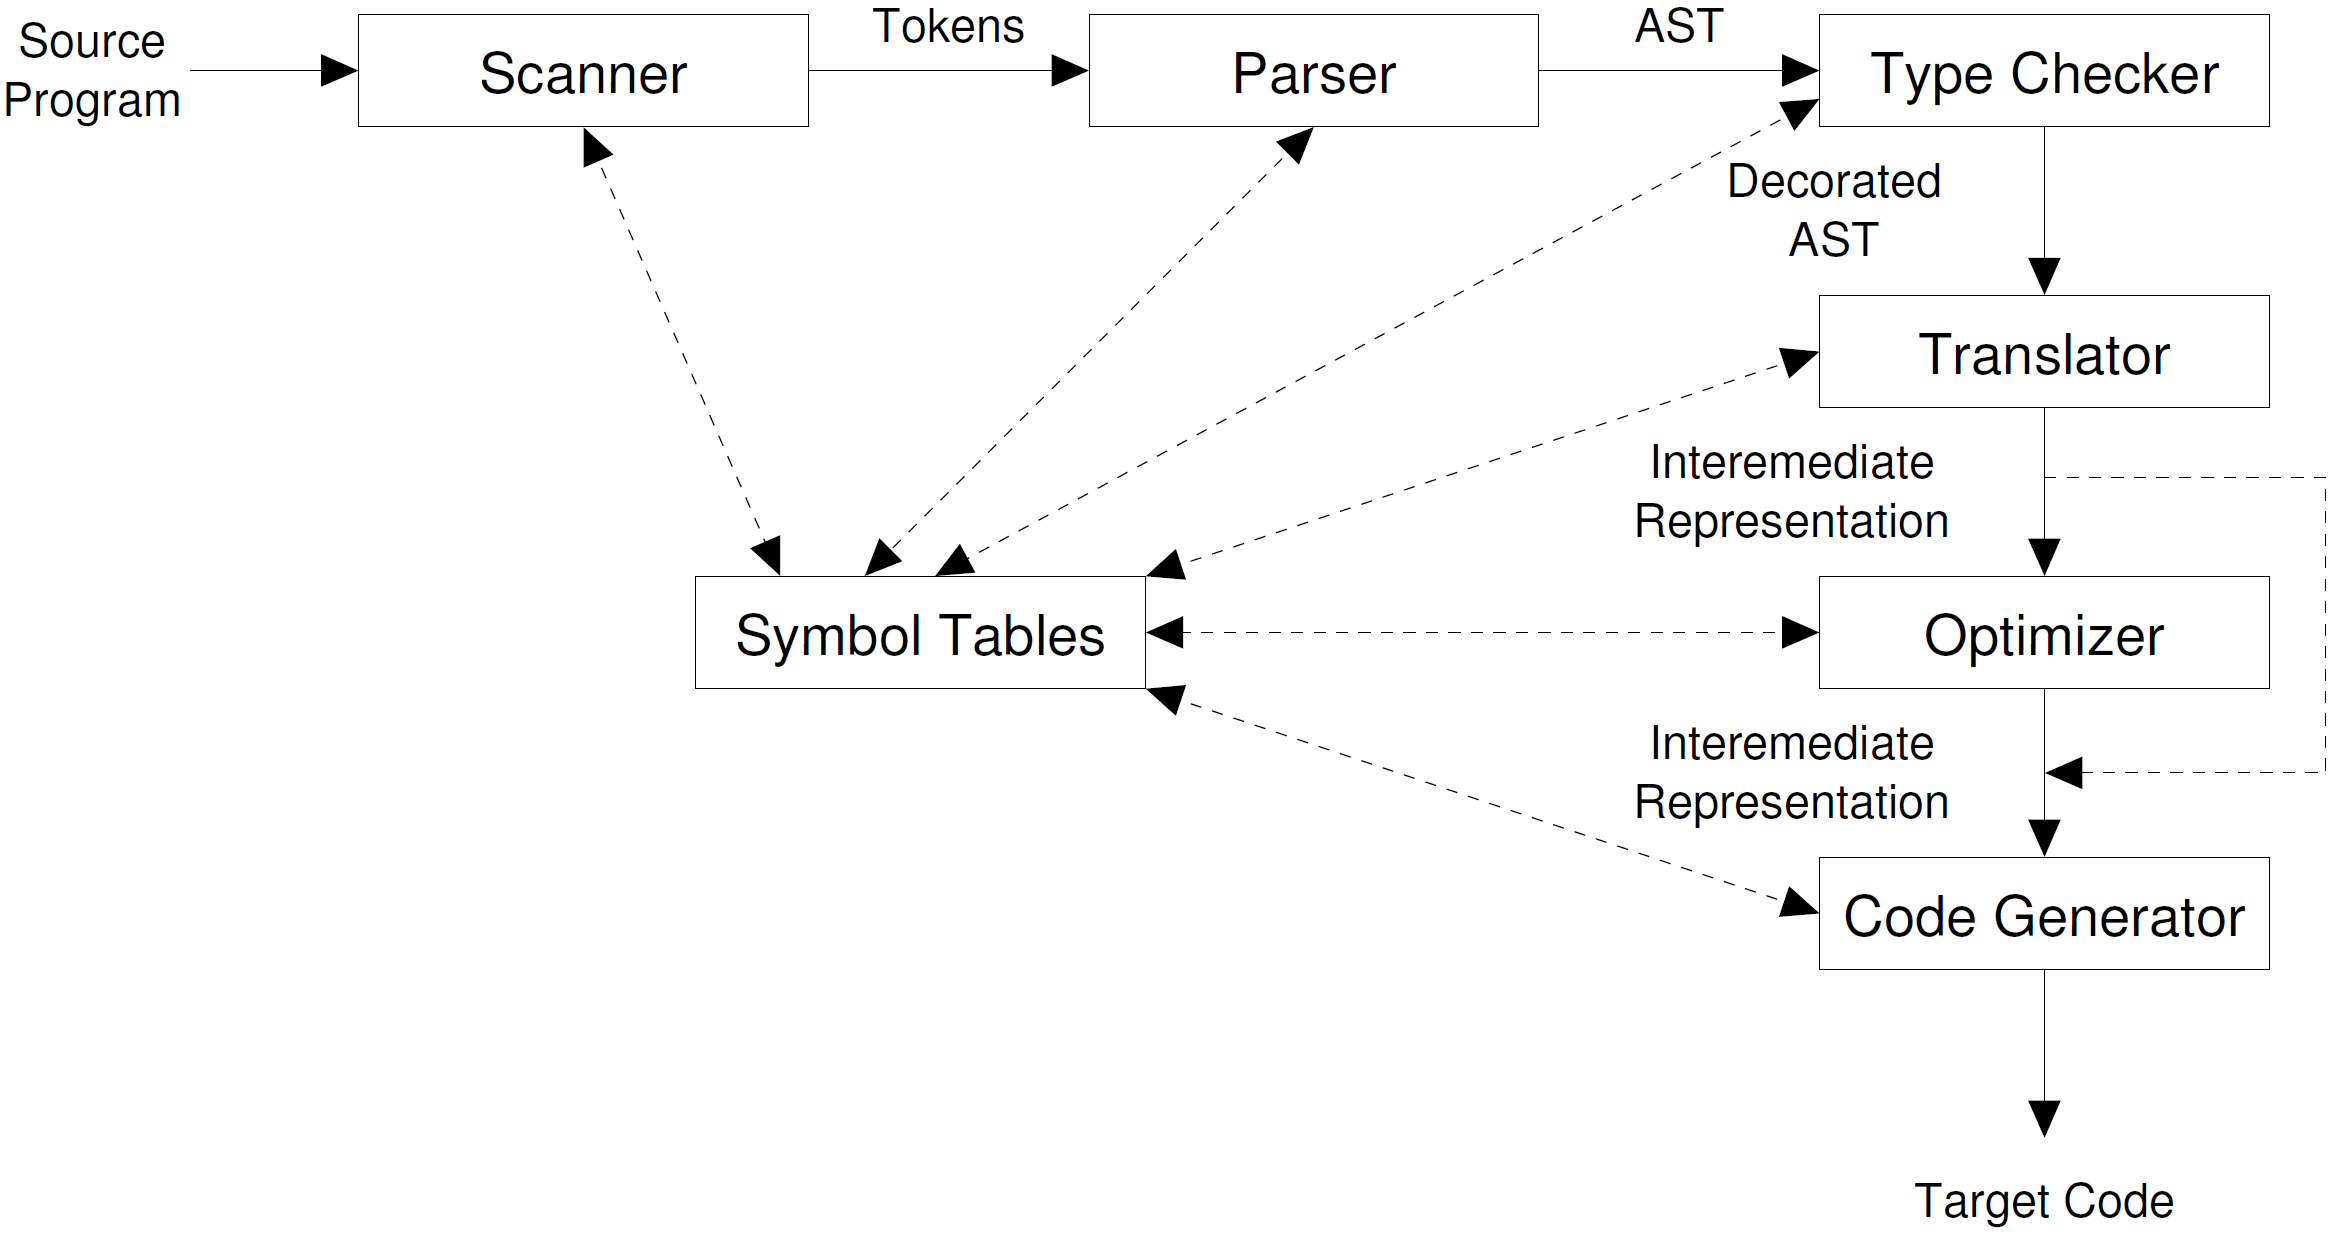
\includegraphics[width=0.8\textwidth]{figures/Full_Compiler.png}
    \caption{A textbook example of a compiler~\cite{CraftingCompiler}}
    \label{fig:generalcompilermodel}
\end{figure}


The target code is often low-level code for a particular system or runtime, but not always. When the target code is another high-level language, the process is also called transpilation. The Arc language is used for programming Arduinos, and so the compiler has to either generate Arduino-specific machine code or transpile it to the high-level Arduino language. Because the Arc language leverages the Protothreads library and its concurrency model for the Arduino, it makes sense for the Arc compiler to be a transpiler.

The Arc compiler follows many of the steps of the general model. Figure~\ref{fig:arccompilermodel} models the Arc compiler with some essential details.


\begin{figure}[htb!]
    \centering
    \begin{tikzpicture}[node distance=3cm]
        \begin{scope}[node distance=3cm,local bounding box=clusterA]
            \node (a) [state] {Scanner} node[below,scale=.7, xshift=60,yshift=-20]{Antlr};
            \node (b) [state, right of=a] {Parser};
            \draw[arrow, ->] (a) -- node[above,scale=.70,align=center]{Tokens} (b);
        \end{scope}
        \begin{scope}[node distance=3cm,local bounding box=clusterB]
            \node (c) [state, shift={($(b.east)+(2.3cm,0)$)}] {Type checker} ;
            \node (d) [state, shift={($(c.south)+(0,-1.5cm)$)}] {Scope checker};
        \end{scope}
        \node(clusterA_g)[cluster,fit=(clusterA)]{};
        \node(clusterB_g)[cluster,fit=(clusterB)]{};
        \node (q) [state, below of=clusterA_g] {Symbol table};
        \node (e) [state, shift={($(d.south)+(0,-1.5cm)$)}] {Code generator};
        \node (f) [shift={($(e.south)+(0,-1cm)$)}] {Target code};
        \node (start) [shift={($(clusterA.west)+(-2cm,0)$)}] {Source code};
        \draw[arrow, ->] (start) -- (clusterA_g);
        \draw[arrow, ->] (b) -- node[right,scale=.70,xshift=-16,yshift=7]{AST} (c) node[below,scale=.7, xshift=-30,yshift=-25, align=left]{Contextual\\ analysis};
        \draw[arrow, ->] (c) -- node[right,scale=.70,align=center]{AST} (d);
        \draw[arrow, ->] (d) -- node[right,scale=.70,align=center]{AST} (e);
        \draw[arrow, ->] (e) --  (f);
        \draw[arrow, dotted, <->] (q) --  (clusterB_g);

    \end{tikzpicture}
    \caption{The Arc compiler model.}
    \label{fig:arccompilermodel}
\end{figure}


Figure~\ref{fig:arccompilermodel} shows how the source code is first scanned into tokens and then parsed into an \gls{ast}. \gls{antlr} generates the lexer and parser for this from our grammar, hence the box around the scanner and parser. The \gls{ast} is then type-checked and scope-checked. The type and scope check rules are explained in more detail in section~\ref{sec:contextualconstraints}. Once the transpiler has done all of the necessary checks on the source code, it is ready to generate the Arduino code, which is also the final step of the compiler. The target code is now ready for the Arduino bases on the source code.
\section{Lexer and parser generation}

%what the lexer and parser is
%differences
%how it is used
%why it is used
%how we generate them
%alternatives
This section will briefly cover how the lexer and parser for Arc has been implemented, and what alternatives could have been used.

For Arc, \gls{antlr} has been used, for creating the grammer and also to generate both the lexer and parser. From writing the grammar, is was possible for \gls{antlr} to generate the lexer, parser and more.\cite{Parr2014} This made \gls{antlr} highly effective for designing Arc, as small changes to the grammar could easily be made, without having to re-create the lexer and parser everytime. Instead only the grammar had to be changed, and \gls{antlr} would generate a new lexer and parser, based on the new grammar.

The grammar was made in a file called 'arcv2.g4' which is an \gls{antlr} file, that \gls{antlr} recognizes and also the lexical rule were made in a file called 'lexerRules.g4'. With these files, \gls{antlr} could generate all needed files for the parser, the lexical analyzer, and other supporting files. These files can be seen in the image \ref{fig:lexerandparserfiles}

\begin{figure}[htb!]
    \begin{center}
        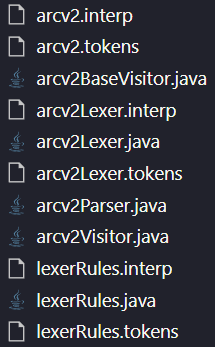
\includegraphics{figures/lexerAndParserFiles.png}
        \caption{Files generated for Arcs parser and lexical analyzer}
        \label{fig:lexerandparserfiles}
    \end{center}
\end{figure}

Figure \ref{fig:lexerandparserfiles} shows all files that \gls{antlr} generates, from the grammar rules and lexical rules. The file 'arcv2Parser.java' is the parser.\todo[]{Describe how the parser works and how it is used. Show code example!}


Another option to this could have been by writing out both the parser and lexer by hand, this could be very educational, as creating our own parser and lexer, would give in-depth knowledge of how they each work. But this would increase the time needed to create Arc considerably as, as mentioned previously, any minor change made in the grammar, would also mean going through the lexer and parser to fix them accordingly. This could lead to time wasted, which is a limiting factor for this project. Therefore it was decided to use the obviouse solution, to use the tools that readily avaliable. For this reason in particular, using \gls{antlr} to generate the lexer and parser for us, was the obviouse choice. 



\todo[inline]{Consinder adding examples of how we specifically have done it and discuss the files generated}

%The lexer, also called a lexical analyzer or scanner, takes a character stream and turns it into tokens. Tokens are a representation of something in a language, such as a num in Arc would be a token, that represents numbers. The lexer recognizes and can discard tokens of the character stream, so that the parser can ignore them. This includes tokens such as comments and whitespaces, that the parser does not need to concern itself with. If the lexer did not discard these tokens, that parser would constantly have to check for them. These tokens are then passed to the parser, that makes syntatic sense of them. It compares the tokens and their structure to the grammar of the specific language.\cite{Parr2014}



\section{Visitor pattern}\label{sec:visitorpattern}\feedback{We still working on this section, and unsure what }
This section will briefly discuss what the visitor pattern is, how it is used in Arc, and why it is used. ANTLR provides two methods of traversing a \gls{cst}, listeners and visitors. 

The listener pattern, is not responsible for calling methods to traverse the tree. ANTLR generates enter and exit methods for each rule, these methods are then called when the walker encounters a node. The benefits of using the listener pattern, is that it is automatic, and the methods created do not have to explicitly visit all their child nodes\cite{Parr2014}. \feedback{We are unsure of how correct this actually is, taken from: Page 18}

The visitor pattern, is a method used to traverse the \gls{cst} in a specific manner, where methods are used to visit each child node. By using the visitor pattern, there is more control of how the traversal of the \gls{cst} is done, and how much of the \gls{cst} is visited. ANTLR can generate a visitor interface, this interface is created from Arcs grammar, and creates all the needed visitor methods. These act as boilerplate for Arcs needed visitor methods, that can then be written out to do excatly as needed\cite{Parr2014}. 

For Arc there is made use of the visitor pattern, because it is not neccecary, for Arc, to visit all nodes, since for some of them it is know what will follow. It is also the more secure option, as it gives the option to be more specific about what happens for each node. This is especially good for futureproofing, as there might be certain things that had not been prdicted, and can therefore be specifically fixed.


%Options
%pros and cons of both
%How is it used
%How do we use it


%Vi vil ikke altid ind i alle noder, fordi det ikke er nødvændigt
%Det er sikre valg, da vi kan være specifikke for hver node, hvis der er noget vi ikke har forudset
%Future proof

\section{Scoping}\label{sec:scoping}
Scoping describes where variables are visible, meaning when a variable can be referenced or assigned. This is an important part of a programming language, since identifiers often are reused, such as i for an iteration. Because of this, scoping is used to differ variables from eachother and also to either allow references to variables or to inhibit reference. For this there are two general types of scoping, dynamic and static.

Static scoping, means that the scope of variabels is determined staticly, meaning it is done before execution of the program. Static scope is used in many languages, including C and C\#. Static scoping is said to be more readable, since the code often shows directly the value of the variable. When a reference to a variable is found, following previous references and finally the assignment to that variable, the value of that variable can be determined. An example of static typing, can be seen in Listing~\ref{lst:scopeexample}.

Dynamic scoping, means that the scope of variabels is determined during run time of the program. Dynamic scope is used in languages including Perl and Common Lips. Dynamic scoping works by using the calling sequence of subprograms to determine the value of eks. a varible. Because of this it cannot be determined staticly as static scoping, and mus tbe done during run time. Dynamic scoping decreases readability of the code, since it can be difficult to know the exact calling sequence of subprograms that contain references to a variable~\cite{Sebesta2016}. An example of how dynamic scoping works, can be seen in Listing~\ref{lst:scopeexample}.\todo{Seems more relevant to the section on language design instead. This section should be about the concrete implementation of Arcs scoping rules than the general ideas of scoping.}

\begin{listing}[htb!]
    \begin{minted}{C}
        int a = 5;

        int fun1(x){
            return x + a
        }
        int fun2(){
            a = 10;
            return fun1(10);
        }
        print(fun2());
    \end{minted}
    \caption{An example of how static and dynamic scope differs}
    \label{lst:scopeexample}
\end{listing}

When using static scoping, Listing~\ref{lst:scopeexample} will print '15', because of the variable a assigned in the beginning being a global variable, and fun1 using that with the x given as it's parameter. Compared to dynamic scoping where there would be printed '20', this is because of the previously mentioned calling sequence. The variable 'a' is assigned to '5', but then in fun2() it is updated to '10' and this value is then used in fun1().

Arc uses static scoping, as it more simple to read and understand for users, and C++ uses a variant of static scoping. Because of this it makes sense for Arc to also a simillar scoping.

In the implementation the creation of the different scopes is primarily archieved through Block structure we use in our syntax. The visitation of this structure is when we push and pop the stack of scopes. This can be seen in Listing~\ref{lst:VisitBlock} Where the visitor visit this node we first push to the context then visit its children and Afterwards we pop this scope that is no longer needed.

\begin{listing}[htb!]
    \begin{minted}{java}
    public AST_node visitBlock(arcv2Parser.BlockContext ctx) {
        symbolTable.push();
        AST_node block = new Variable_declaration_node("block");
        List<arcv2Parser.StatementContext> list = ctx.statement();

        for (arcv2Parser.StatementContext statementContext : list) {
        visit(statementContext);   
        }
        symbolTable.pop();

        return block;
    }
    \end{minted}
    \caption{VisitBlock from our evalvisitor}
    \label{lst:VisitBlock}
\end{listing}

Our Scoping rules are implemented everywhere in our semantic visitor, an example of how it works can be seen in Listing~\ref{lst:ScopeImplementationExample} where it can be seen that our forloop use a call to our symbolTable to check if the identifier given as input has been declared. This archieved using the get function showed earlier, which returns null if it does not exist.

\begin{listing}[htb!]
    \begin{minted}{java}
    @Override public AST_node visitForloop_statement(arcv2Parser.Forloop_statementContext ctx) { 
        ...
        SymbolHashTableEntry entry = symbolTable.get(ctx.IDENTIFIER(1).getText());
        if (entry == null) {
            throw new RuntimeErrorException(null, "this identifier '" + ctx.IDENTIFIER(1).getText() + "' does not exist" );
        }
        ...
    }
    \end{minted}
    \caption{The SymbolHashTableEntry class}
    \label{lst:ScopeImplementationExample}
\end{listing}



%What is scoping
%Blocks
%Types of scoping
%Pros and cons of the two
%What does Arc use
\section{Type checker}
This section will discuss the type checker for Arc, how it is structured and also show examples of how it works.

The type checker verifies that operands of an operator are of compatible types, and if not, throws an error, with an error message for the user to use to fix the issue \cite{Sebesta2016}. It does this by walking through the \gls{cst} from the bottom-up, with a visitor pattern \cite{Parr2014}. An example of the type checker throwing an error would be the case where a user tries to use the plus operand on a num and a char, this will throw an error to the user telling them, that this operation is not valid in Arc.

There are two ways to type check, static and dynamic type checking. Static type checking works on compile time, dynamic type checking is done during run time. Usually it is better to use static type checking, as it catches errors earlier compared to dynamic type checking, and is less costly \cite{Sebesta2016}. Altough dynamic typing allows for more flexablility when writing code, as in languages such as Python where types are not needed to be declared, but simply values are to be given.

In Arc there will be made use of a static type checker, this is because the language that Arc transpiles to is C++ which is a staticly typed language. For this reason it makes sense for Arc to also be a staticly typed language, so it can be easily used with the Arduino, which uses a language that is a subset of the C++ language. \todo{indsæt evt ref til at Arduino bruger C++} Combined with the previously mentioned benefits of using a staticly typed language, it seemed like the obviouse decision to have Arc be a staticly typed language. Although an argument could be made that Arc should be made a dynamicly typed language, since often dynamicly typed languages, such as Python, tend to be faster to write code in. Since time is a limiting factor for our definition of a hobbyist, it would make sense to make a language that encourages less time spent writing code. But since Arc is only made to work with simple concurrency, this time spent on writing code, might not give as much of a gain, as in a standard language. \todo{This just sounds like bullshit -gustav "true"}

\begin{listing}[htb!]
    \begin{minted}{java}
        SymbolHashTableEntry entry = symbolTable.get(ctx.IDENTIFIER().getText());
        

        //TODO  this needs to handle arrays (should we even allow array assignment)
        AST_node expression = visit(ctx.expression(0));

        if (entry == null) {
            throw new RuntimeException(" this varible '" + ctx.IDENTIFIER().getText() + "' does not exist");
        }
        else if (entry.Mutability != true) {
            throw new RuntimeException(" this varible '" + ctx.IDENTIFIER().getText() + "' is not mutable and therefore cannot be assigned to");
        }
        else if (entry.Type !=  expression.type) {
            throw new Expression_type_exception("the assingment expression has bad typing");
        }
        else{
            symbolTable.insert(entry);
        }
    \end{minted}
    \caption{Code snippet of Arcs type checker}
    \label{lst:typecheckerexample}
\end{listing}
\todo[inline]{Feel like it is missing a function name}
\todo{this is actually a bad example as it shows too much you talk about alot of checks that arent type check like scope cheks}
\ref{lst:typecheckerexample} shows am example of Arcs typechecker. This example shows the part of the typechecker, handles assignments. It does this by creating 'entry' of the class SymbolHashTableEntry and assigns it to the contents of a ctx file\tode{yeah, naw. thats not whats happening were creating an entry and assigning to it the result of a lookup in the symbolTable based on the IDENTIFIER that were assigning to.}. Then it creates 'expression' of the AST\_node class, and uses a visitor method to assign it to the first expression of the \gls{cst}\tode{this is closer. here were creating a ast nodes and assingning it the result of a visit to a expression. and in our visitor a visit always returns a ast node}. It is then evaluated in a sequence of if statements, to ensure that the assignment is a legal action in Arc. First checking if the entry even exists, then if the entry is mutable and finally checking if the types of the entry and expression are equvilant. If the entry passes all the checks, it is then inserted into the sybol table. If it does not pass one of the checks, an exeption is thrown and a relevant error message is given.
\todo[inline]{Entire paragraph has to be checked to ensure it is correct}


%dynamic vs static typechecking
%formal definitions som cagala?
%Why is it important to have a typechecker
%argument could be made that a dynamic typed language would be better for hobbyists since time is a limiting factor for them, and in general dynamicly typed languages are faster to write code in.
\section{Code Generation}\label{sec:codegeneration}
This section will explain the code gen part of the compiler. In this part of the implementation, the target
code is generated. The target code is the Arduino language, which is essentially c/c++ with some Arduino constructs. The code is generated using another visitor pattern similar to the one we use for semantic analysis. It follows the divide and conquer principle and uses the antlr generated \gls{ast}. It then generates the code going through the \gls{ast} and passing the generated code between the nodes using our CodeGenStringObject.

\begin{listing}[htb!]
    \begin{minted}[label=CodeGenStringObject class definition]{java}
    public class CodeGenStringObject {
    public String GlobalScope = "";
    public String Setup = "";
    public String Loop = "";
    public String Type_Coverter (String input){
        if(input.equals("mut num") || input.equals("num" )){
            input = "float";
        }
        if(input.equals("mut char")){
            input = "char";
        }
        if(input.equals("mut bool")){
            input = "bool";
        }
        return input;
        }
    }
    \end{minted}
    \caption{CodeGen object used in code generation.}
    \label{lst:code gen object}
\end{listing}

We use the CodeGenStringObject because a node sometimes will generate code in 3 different places of the final code at once. Hence we have made an object containing three different strings and a method. The three strings each correspond to one of the three areas that can be generated to the three sections, GlobalScope, the Setup structure, and the loop structure. This makes it possible to do all code-gen simply in a single visit of the three because it's unnecessary to keep track of 3 different placements in the file and switch between writing in them. The final code gen is done by using the final CodeGenStringObject and simply inserting the three strings into the file in order. \todo{this needs to be more clear, and use an example to show it} The method in CodeGenStringObject is simply used in code-gen to rewrite the types that we have in the input to the corresponding types in c++.

The visitor pattern is very similar to the one used for type checking, scope checking, etc. This is because they are all extensions of the arcv2basevisitor. This is possible because they're using the same Antlr generated \gls{ast} as input. A custom \gls{ast} is not created because it would look very similar to the one Antlr would generate because our grammar generally creates a quite shallow tree, so the \gls{ast} would not be very different in structure. It would also make it necessary to do a lot of reimplementing a lot of methods and data structures that antlr \gls{ast} has baked in. Therefore we keep using the antlr \gls{ast} since there isn't a lot of upside to making a new one. \todo{does this sound convincing?}


In figure \ref{lst:codegenexpression} we see a simple example of how The code gen visitor works. Here we see it first creates two objects of the class CodeGenStringObject shown earlier. One is named cpp, which stands for c + +, and one is named temp since it is temporary and does not get returned out of the method. Then we assign temp the result, and the global scope of this object is then added to cpp. Only the global scope is added since we know only different expressions can exist within an expression, and none of our expressions add to anything other than the global scope. Then we use the result of ctx.plus to check if we should add a plus or minus to cpp. Ctx.plus equals either a plus terminal or null if it doesn't exist; hence this is possible. In the end, we do the same thing again with the visit, just with the second expression, which is then added to cpp, and cpp is returned to the parent of this node. We don't check if more exist because only two can exist in a plus-minus ctx. So basically, this visitor visits a node, adds the result of visiting its children to it, and then returns it to its own parent, which is how our code-gen works.


\begin{listing}[htb!]
    \begin{minted}[label=CodegenVisitor.visitPlusMinusExpression]{java}
    public CodeGenStringObject visitPlus_minus_expression(arcv2Parser.Plus_minus_expressionContext ctx) {
        CodeGenStringObject cpp = new CodeGenStringObject();
        CodeGenStringObject temp = new CodeGenStringObject();
        temp = visit(ctx.expression(0));
        cpp.GlobalScope += temp.GlobalScope + " ";

        if (ctx.PLUS() != null) {
            cpp.GlobalScope += "+ ";
        } else {
            cpp.GlobalScope += "- ";
        }
        temp = visit(ctx.expression(1));
        cpp.GlobalScope += temp.GlobalScope;

        return cpp;
    }
    \end{minted}
    \caption{code gen object used in code gen}
    \label{lst:codegenexpression}
\end{listing}


A different interesting part of the code-gen visitor is the task declaration visit which is visible here\ref{lst:codeGenTask}.
This one has a bit more happening. The first part until line??? describes the creation of the cpp CodeGenStringObject and all the things that should be added to the global scope every time a task is declared. It also creates a name for the thread, which will be used in c++. This is necessary because the tasks in arc do not have names. These names are generated generically based on a counter function which can be seen at the button, so they end up being named pt0thread, pt1thread, etc.
That means all the things need to be inserted to create a protothread. Afterward, we see three control structures, an if, else if, and an else, which describe the three different ways we describe a task.

Firstly in line??, we have an if statement that, similarly to the previous example, checks if there is an every and if there is, we enter the if statement. Inside First that happens is the creation of a list of all the statements that are the immediate children of task declaration. This list is then iterated through, and the result of the visits to the individual children are added to the cpp in order. This Finishes with adding what is essentially a call to a protothreads function sleep that sleeps the thread for the amount of time specified in the Number, which corresponds only to every because it only exists if there is an every.

Second is the case where we use a when. In that case, we add an if statement inside of the protothread and insert the product of a visit to the boolean expression that we know has to exist if there is a when per our grammar. On line??, we again see the construct used to add the statements.

The Third else case is just the same statement iteration without anything extra.


how it works with example -tasks
\begin{listing}[htb!]
    \begin{minted}[label=CodegenVisitor.visitTaskDeclaration]{java}
    @Override
    public CodeGenStringObject visitTask_declaration(arcv2Parser.Task_declarationContext ctx)
    {
        CodeGenStringObject cpp = new CodeGenStringObject();
        String ptName = "pt" + Integer.toString(get_task_number());
        String ptNameThread = ptName + "thread";

        cpp.GlobalScope += "pt " + ptName;
        cpp.GlobalScope += ";\n";
        cpp.GlobalScope += "int " + ptNameThread + "(struct pt *pt) { \n PT_BEGIN(pt);\n for(;;){ \n";

        if (ctx.EVERY() != null) {
            List<StatementContext> list = ctx.statement();
            for (StatementContext statement : list) {
                cpp.GlobalScope += visit(statement).GlobalScope;
            }
            cpp.GlobalScope += "\nPT_SLEEP(pt, " + ctx.NUMBER().getText() + ");\n";
            cpp.GlobalScope += "\n}\n";
        } else if (ctx.WHEN() != null) {
            cpp.GlobalScope += "if (" + visit(ctx.expression()).GlobalScope + ") { \n";
            List<StatementContext> list = ctx.statement();

            for (StatementContext statement : list) {
                cpp.GlobalScope += visit(statement).GlobalScope;
            }
            cpp.GlobalScope += "\n}\n";
        } else {
            List<StatementContext> list = ctx.statement();
            
            for (StatementContext statement : list) {
                cpp.GlobalScope += visit(statement).GlobalScope;
            }
            cpp.GlobalScope += "\n}\n";
        }
        cpp.GlobalScope += "PT_END(pt);\n}";
        cpp.Setup += "PT_INIT(&" + ptName + ");";
        cpp.Loop += "PT_SCHEDULE(" + ptNameThread + "(&" + ptName + "));";

        return cpp;
    }
    \end{minted}
    \caption{Code generation of task declarations.}
    \label{lst:codeGenTask}
\end{listing}

\begin{listing}
    \begin{minted}[label=CodegenVisitor.getTaskNumber]{java}
        private int count = 0;
        public int get_task_number() {
            int temp = count;
            count += 1;
            return temp;
        }
    \end{minted}
    \caption{Keeping track of the number of tasks.}
    \label{lst:codeGenTaskNumber}
\end{listing}







\section{MOVE ME EVENTUALLY}
This section contains text that has to be moved to proper sections.

\subsection*{Arc implemementation of the sample project}
The sample project implemented in Arc.

\begin{listing}[htb!]
    \begin{minted}[label=Arc example]{text}
        #pin BUTTON_PIN(12, OUTPUT);
        mut num buttonState = 0;
        mut bool ledState = HIGH;

        task(bool ledState) every 1000 {
            ledState = not ledState;
            digitalWrite(LED_BUILTIN, ledState)
        }

        task(num buttonState) {
            buttonState = digitalRead(BUTTON_PIN);
            Serial.Println(buttonState);
        }
    \end{minted}
    \caption{Project example implemented in Arc, assuming print is possible.}
    \label{lst:arcexample}
\end{listing}
